\documentclass{acm_proc_article-sp}

\usepackage{color}
\usepackage{graphicx}
\newcommand{\TODO}[1]{\textcolor{red}{{\bf TODO:} #1}}
\newcommand{\checkme}[1]{\textcolor{red}{\textbf{#1}}}



\usepackage{microtype}
\usepackage{placeins}
\begin{document}
\addtolength{\topmargin}{-.5in}
\addtolength{\textheight}{.7in}
\addtolength{\oddsidemargin}{-.25in}
\addtolength{\evensidemargin}{-.25in}
\addtolength{\textwidth}{.5in}
\addtolength{\topsep}{-3pt}
\linespread{.94}

\title{Pomace: A Grappa for Non-Volatile Memory \vspace{-.2in}}
\authorinfo{Jacob Nelson$^{\dagger}$,
  Brandon Holt$^{\dagger}$,
  Brandon Myers$^{\dagger}$,
  Preston Briggs$^{\dagger}$,
  Luis Ceze$^{\dagger}$,
  Simon Kahan$^{{\dagger \ddagger}}$,
  Mark Oskin$^{\dagger}$
}{\textdagger University of Washington, \textdaggerdbl Pacific Northwest National Laboratory}{
  \{nelson, bholt, bdmyers, preston, luisceze, skahan, oskin\}@cs.washington.edu \vspace{-1in}
}

\maketitle
\begin{abstract}
We revisit Grappa, our software platform that scales in-memory irregular
applications on mass market clusters.
We contemplate options for adapting Grappa to use non-volatile memory technologies.
\end{abstract}
\vspace{-.1in}

\section{What is Grappa?}
Grappa is a latency-tolerant runtime system for off-the-shelf clusters
that targets in-memory irregular applications, such as interactive graph analytics.  These
applications are notoriously difficult to scale up due to
data-dependent execution and memory access behaviors. The resulting
irregularity in computational demands hinders efforts to balance load
and to maintain spatial and temporal locality.  Resulting
inefficiencies are exacerbated at scale, as wasted energy rises with
the number of idling nodes, undersized network packets, and cache
misses.  Consequently, few irregular applications today make good use
of high-performance computers.  Those that do, use complex, application-specific techniques to overlap computation with communication and are
developed by expert programmers, who are in short supply.

Yet, there is increasing demand for irregular applications. Evidence
is the growing number of publications, conferences, and companies
focused on graph benchmarks, semantic databases, machine learning, and
``big data'' discovery. Grappa aims to mitigate the inefficiencies plaguing development and execution of these important applications. The system (Figure~\ref{fig:grappa}) has three main software components:

\FloatBarrier
\begin{figure}[t]
\begin{center}
  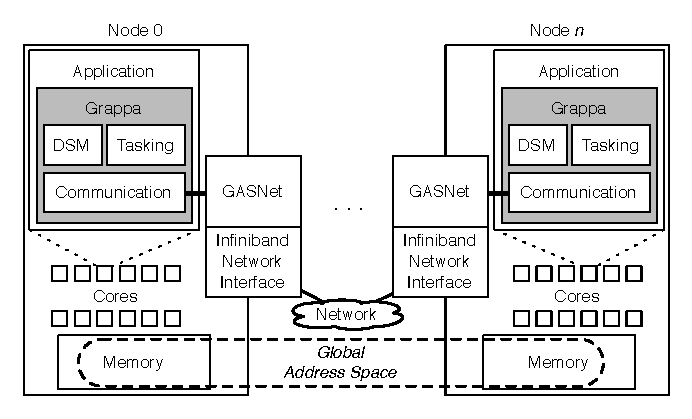
\includegraphics[width=0.95\columnwidth]{../asplos13/figs/system-overview}
\begin{minipage}{0.95\columnwidth}
  \nocaptionrule\caption{\label{fig:grappa} Grappa system overview}
\end{minipage}
\vspace{-5ex}
\end{center}
\end{figure}


\begin{description}

\item [Tasking system.] Our tasking system supports lightweight
multithreading to tolerate communication latency; it also supports global distributed
work stealing (i.e., tasks can be stolen from any node in the system), which
provides automated load balancing.  Grappa thus tolerates many
microseconds of latency by multiplexing thousands of tasks per x86 core.

\item[Communication layer.] Modern mass market networks
support high bandwidth only for large messages, but irregular applications
frequently issue small requests.   Our communication layer aggregates these small requests into larger messages to better exploit network bandwidth, targeting 100 million 8-byte remote references per second per node.  Aggregation is largely invisible to the application programmer.

\item[Distributed shared memory.] Our \textls*{\small DSM} system provides support for
fine-grain access to data anywhere in the system. It supports synchronization
operations on global data, explicit local caching of any memory in the system,
and support for operations on remote data (delegating operations to the data's owner node).
By tight integration with the tasking system and the
communication layer, our \textls*{\small DSM} system offers high aggregate random-access bandwidth to remote data.

% software developer but helps to improve network performance when applications read and write only small pieces of data.

\end{description}
Grappa thus facilitates
expression of fine-grained task parallelism at the application
programming level, employing that concurrency as needed to sustain throughput in the presence of long latency operations and to better utilize mass market networks.  Programmers attend only to expressing the parallelism in their program, not to scheduling it.  While similar latency-tolerance and aggregation techniques can be manually coded into some
applications, Grappa relieves the programmer of this burden.  In
addition, Grappa provides an \textls*{\small API} for reader-writer lock semantics for the
purpose of manipulating a local copy of any contiguous portion of the
shared address space, enabling programmers to exploit spatial and
temporal locality while maintaining a consistent global view.  With
these features, we have demonstrated performance on mass market systems
for highly irregular applications approaching that of the Cray \textls*{\small XMT}~\cite{feo:xmt}, a
fully custom system.

\subsection{What's the problem?}

While Grappa's current design scales to the limit of available network
bandwidth, it does so only for applications whose working set resides
in \textls*{\small RAM}\@.  Unfortunately, provisioning systems with petabytes of \textls*{\small RAM} is
costly, energy inefficient, and likely to increase the time to prepare
for and recover from faults.

Emerging non-volatile memory technologies offer an alternative strategy:
place the entire data set on Flash or \textls*{\small PCM}, and
%% use Grappa to tolerate the latency either directly, much in the same
%% way as it is used now to tolerate network latency, or indirectly when transferring blocks of working-set
%% data into \textls*{\small RAM}. This could save energy per available byte and allow
%% faster fault recovery with most of the data preserved in non-volatile memory.
use Grappa to tolerate the access latency. This could save energy per available byte and allow
faster fault recovery with most of the data preserved in non-volatile memory.

Prior work only partially explores this potentiality. GraphChi~\cite{graphchi:osdi12}
represents a class of approaches that use windowing methods in the
irregular application space, structuring the data on secondary storage
to support filling \textls*{\small RAM} with multiple interrelated subblocks sufficient
for each of a series of phases of computation.  Such approaches are
algorithmically efficient only when each successive phase requires
access to the entire data set.  Pearce et al.~\cite{magt:2010} address this limitation by
introducing support for asynchronous computation on graphs under the
assumption that \textls*{\small RAM} is sized to accommodate data structures
proportional to vertex-count, still leaving edges on non-volatile
storage.  In addition, both methods apply only to single node systems:
Grappa provides a global view of memory on multinode systems.

\section{Applying non-volatile memory to Grappa}
The natural point of integration for non-volatile memories in Grappa
is to store the global distributed shared heap in non-volatile memory, since for irregular applications the heap
often holds data that is infrequently modified. All accesses to
this shared heap in Grappa programs are done through an \textls*{\small API}, so this change could be made transparent to the programmer. 

If an 
access is to a chunk of the heap stored in a node's local memory, Grappa issues a prefetch for the address
and context switches to other work while the prefetch is executing~\cite{Nelson:hotpar2011}. If
the access is to memory stored on another node, Grappa issues a
message to that node to request the data and context switches to other
work until the reply arrives. Non-volatile memory would be accessed in
the same way: If a request is to memory stored in non-volatile memory,
Grappa would initiate the request and context switch to other work
until the request had completed.

\subsection{Challenges in using mass market \textls*{\small SSD}\hspace{0.75pt}s}
Grappa's goal is to provide good irregular application performance on
mass market hardware. Unfortunately, mass market \textls*{\small SSD}\hspace{0.75pt}s are
difficult to use directly for three reasons:

%\paragraph{\textls*{\small SSD}\hspace{0.75pt}s assume locality.} In our benchmarks, we find the average request size to be
\noindent{\bf \textls*{\small SSD}\hspace{0.75pt}s assume locality.} In our benchmarks, we find the average request size to be
less than 64 bytes. Today's \textls*{\small SSD}\hspace{0.75pt}s are optimized for reads in the
multi-kilobyte range.  

%\paragraph{\textls*{\small SSD}\hspace{0.75pt}s have a low request rate.} The fastest~\cite{fusionio} can
\noindent{\bf \textls*{\small SSD}\hspace{0.75pt}s have a low request rate.} The fastest~\cite{fusionio} can
perform on the order of 1 million random reads per second, and many
are limited to less than 100K/s. Even the individual flash chips are slow, on the order of 40K/s~\cite{micronFlash}. In contrast, cores may be idle in
Grappa if each node cannot perform 100 million random reads per second of
the global heap. 

%\paragraph{\textls*{\small SSD}\hspace{0.75pt}s have high overhead.} Mass market \textls*{\small SSD}\hspace{0.75pt}s are usually treated
\noindent{\bf \textls*{\small SSD}\hspace{0.75pt}s have high overhead.} Mass market \textls*{\small SSD}\hspace{0.75pt}s are usually treated
as normal disks: accesses must occur through the kernel, incurring a
high context-switch overhead. Grappa depends on user-mode access to
the network layer to avoid this overhead; a similar approach has been applied to \textls*{\small SSD}\hspace{0.75pt}s in recent research~\cite{caulfield:2012}.

\subsection{Exploring the design space}

Previously we discussed the mechanism by which memory references in
Grappa could be issued to non-volatile memory devices. In this
section, we explore a number of different designs for interfacing the
non-volatile memory hardware with Grappa nodes. Each design has
tradeoffs, which we briefly discuss.

For simplicity, we omit discussion of write and erase operations. We
assume a non-volatile Grappa would store frequently written temporary
data in \textls*{\small DRAM} and would use its standard latency-tolerance techniques
to cover the cost of infrequent writes to non-volatile memory.

\subsubsection{Tolerating Flash-based \textls*{\small SSD} latency} 
A natural first step would be to add one or more mass market \textls*{\small SSD}\hspace{0.75pt}s to each Grappa
cluster node, and use Grappa's global memory \textls*{\small API} to expose concurrent
accesses and context switch to tolerate the latency of \textls*{\small SSD}
access. Unfortunately this is unlikely to work well, for two
reasons. First, as discussed earlier, the \textls*{\small SSD} must accept requests at a rate sufficient to
keep the cores busy; current \textls*{\small SSD}\hspace{0.75pt}s
can accept requests at a rate two to four orders of magnitude slower than required.
Second, the \textls*{\small SSD} must be able to support many requests operating in
parallel. Little's Law suggests that if requests take 25 $\mu$s for
the \textls*{\small SSD} to service, and if the node generates requests at a rate of
100 million per second, the \textls*{\small SSD}\hspace{0.75pt}s must support 2500 concurrent
requests. Again, existing \textls*{\small SSD}\hspace{0.75pt}s support orders of magnitude less request concurrency.

We see three ways to address this disparity.

\paragraph{Scaling up the Flash array.}
%\noindent{\bf Scaling up the Flash array}
Existing Flash-based \textls*{\small SSD}\hspace{0.75pt}s are designed for large block requests. An
\textls*{\small SSD} for Grappa could be designed to support high concurrency, small
requests. Where a traditional \textls*{\small SSD} might put multiple Flash chips on
the same bus, or use Flash chips in parallel to build a wider,
high-bandwidth bus, a Grappa \textls*{\small SSD} would try to maximize parallelism by
putting each chip on its own bus. Serial Flash might be used to
minimize pin count requirements, at the cost of some additional
latency. This design could scale to request rates, but the challenge
would be chip count: to support 100 million reads per second, an array of
25$\mu$s flash would require 2500 chips. This is possible, but expensive.

\paragraph{Scaling down the processors.}
%\noindent{\bf Scaling down the processors.}
Alternatively, rather than scaling up the flash array, processors
could be scaled down to match the flash request rate. A low-power
processor with few cores might generate only 1 million references per
%second. This could be satisfied with only 25\,x\,25$\mu$s Flash chips.
second. This could be satisfied with only $25\times 25\mu$s Flash chips. 
%Similar have demonstrated energy-efficient operation in recent research~\cite{gordon:2009}.
There are two problems with this design for our purpose. First, while each node
requires fewer chips, the overall cluster performance goal, and thus
chip count requirement, is the same. Second, low single-threaded performance is detrimental to performance during periods of diminished application concurrency.

\paragraph{Buffering requests to increase locality.}
%\noindent{\bf Buffering requests to increase locality.}
Grappa trades latency for better throughput by aggregating network
communications for better utilization and by migrating synchronization
operations for reduced contention. The same idea could be applied to
increase locality and amortize the cost of Flash accesses. Requests
to nearby flash locations would be bucketed by flash page address for a
limited time. When a sufficient number of requests have arrived for a page
or when the requests time out, a single page request would be issued to the Flash
layer; its result would be used to satisfy the individual requests.

While similar techniques have provided benefit for graph traversal applications in
restricted situations~\cite{magt:2010}, they depend on a sufficient request
density to each flash page to get a benefit. As datasets scale up and machines scale out, this
density may decrease, limiting the benefit of this technique.

For iterative applications where the entire graph is regularly
visited, an windowed approach similar to~\cite{graphchi:osdi12} may
provide more benefit. In this approach, graph data is constantly
streamed between \textls*{\small SSD} and \textls*{\small DRAM}. Requests would wait to execute until the
relevant fragment of the graph is in memory. Request density is not a
concern for these applications; instead, bandwidth between the \textls*{\small SSD} and \textls*{\small DRAM}
is the limiting factor.

\subsubsection{Using future memory technologies}

While Grappa's goal so far has been to leverage mass market hardware, it
is worth exploring the potential benefit of emerging non-volatile
memory technologies like Phase-Change Memory. The advantages of \textls*{\small PCM}
are twofold: first, read latency is much closer to that of \textls*{\small DRAM}, and
second, \textls*{\small PCM} supports finer-grained accesses.

\paragraph{\textls*{\small PCM} as main memory.}
%\noindent{\bf \textls*{\small PCM} as main memory.}
Recent research has explored the use of \textls*{\small PCM} as a main memory
replacement~\cite{pcm:isca09}. Grappa would easily be able to take advantage of such a
development. When a Grappa program references low-locality data,
a prefetch request is issued for that data a few cycles before the
thread is context switched in. A \textls*{\small PCM}-based
Grappa would do the same, but would issue the prefetches earlier to
cover the longer latency of \textls*{\small PCM}.

\paragraph{\textls*{\small PCM} as attached storage.}
%\noindent{\bf \textls*{\small PCM} as attached storage.}
Grappa could also transparently support a \textls*{\small PCM} array in a separate address space (for
instance, on the \textls*{\small PCIe} bus). \textls*{\small PCM} chips available today~\cite{micronPCM} support a
64-bit read in 200 ns; this means that 20 chips acting independently
would be sufficient to reach our target request rate.

Just as in network communications, issuing individual \textls*{\small PCIe} bus
operations for each memory request has too high overhead to get a
reasonable request rate.  Instead, Grappa would delay threads
performing operations in the \textls*{\small PCM} array until it could send a buffer
with enough requests to amortize the overhead. The \textls*{\small PCM} array would
perform the operations and buffer the results. When a sufficient
number have completed, the \textls*{\small PCM} array would write the results to \textls*{\small DRAM}\@,
and one core would deliver the results to the requesting threads,
waking them.

%An ideal array would support limited atomic operations on 64-bit
%words, including increment and compare-and-swap.

This system could be built today, with the only downside being
density: currently available \textls*{\small PCM} chips are significantly less dense
than Flash or even \textls*{\small DRAM}\@. \textls*{\small PCM}'s technology scaling curve suggests that
this will be an ideal solution in the future.

\section{Conclusion}
Efficient execution of irregular applications on large datasets is of
growing importance.  Grappa promises to address this need on mass
market clusters.  Addition of non-volatile storage is a natural
extension of such systems.  We ask, what would developing a Pomace for
Grappa -- a Grappa system exploiting non-volatile memory -- entail and
what capability and efficiency improvements might it bring to Grappa's
application space?  Answering this question is an opportunity for
collaboration between our group and the non-volatile memory research community.


\begin{spacing}{0.8}
\bibliographystyle{abbrv}
\bibliography{paper}
\end{spacing}

\end{document}



